\section{System to Build} \label{sec:promise}

To support the standard RDMA Verbs API used by containers and realize
communications with the best available data-plane mechanism, \sysname needs
to present a RDMA environment to containers and efficiently supports 
the RDMA semantics with multiple data-plane mechanisms. While RDMA has
four interfaces (e.g. Write, Read, Send and Receive), we use Write as an example
to show how \sysname supports this operation with shared-memory and real RDMA.

     \begin{figure}[ht]
     \centering 
%     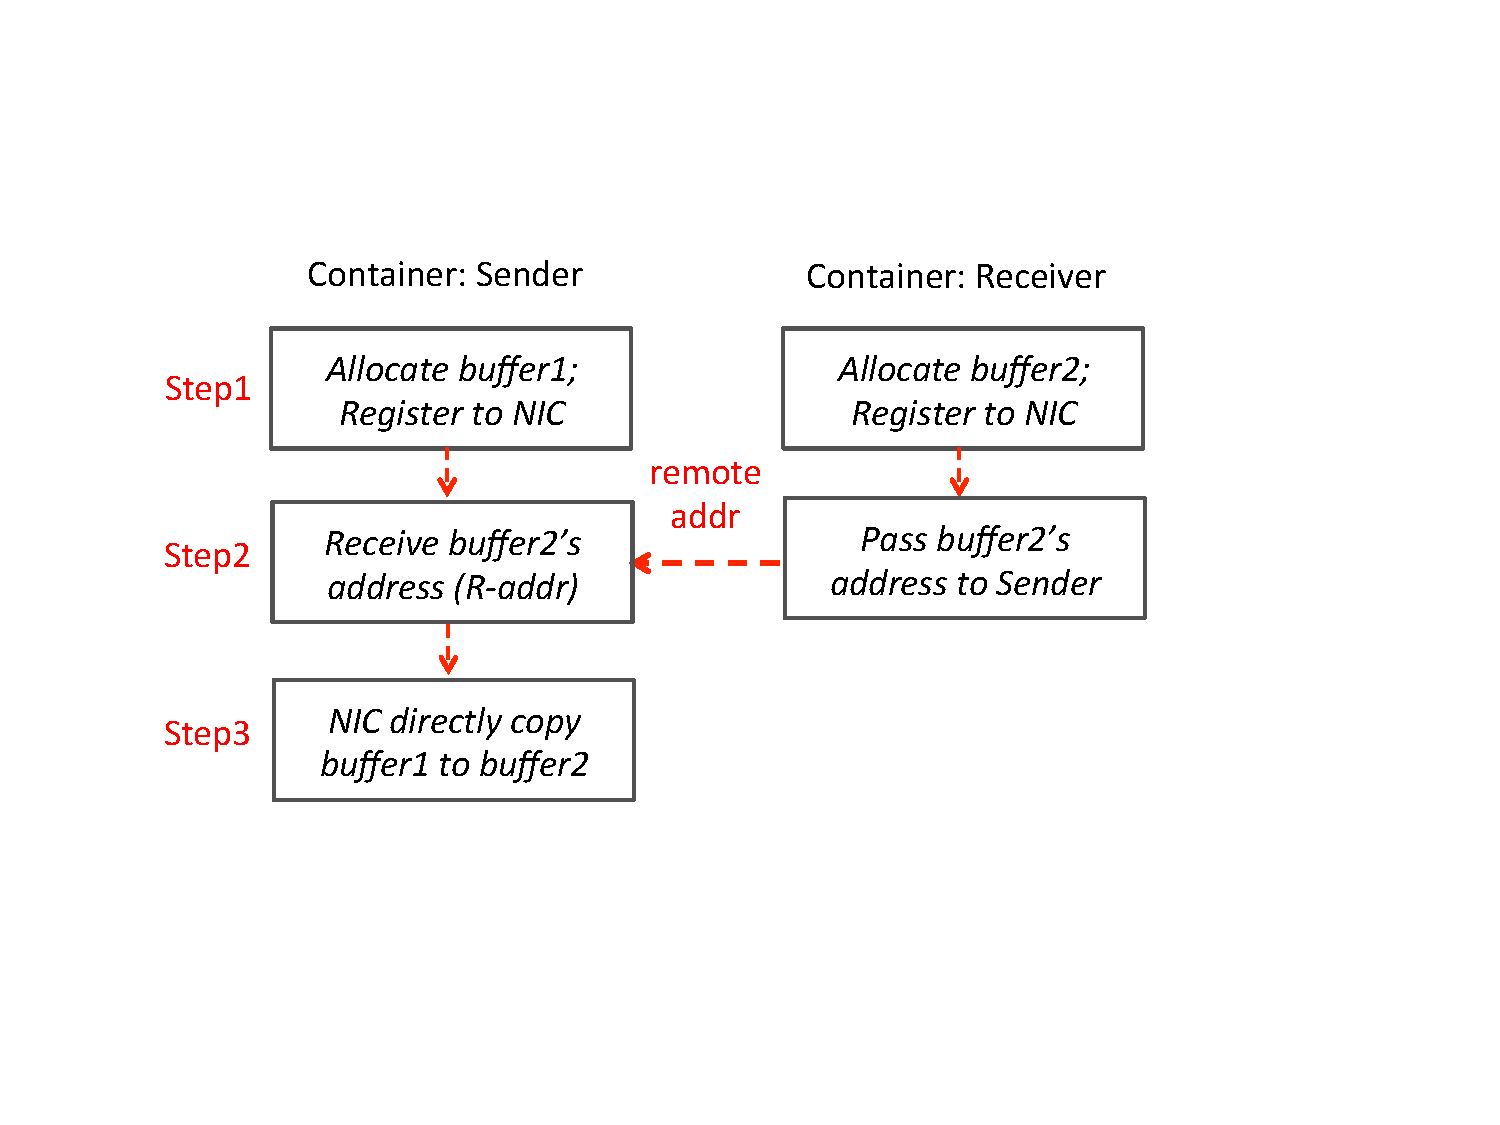
\includegraphics[width=0.45\textwidth]{figures/system/sys_rdma_steps.pdf}
     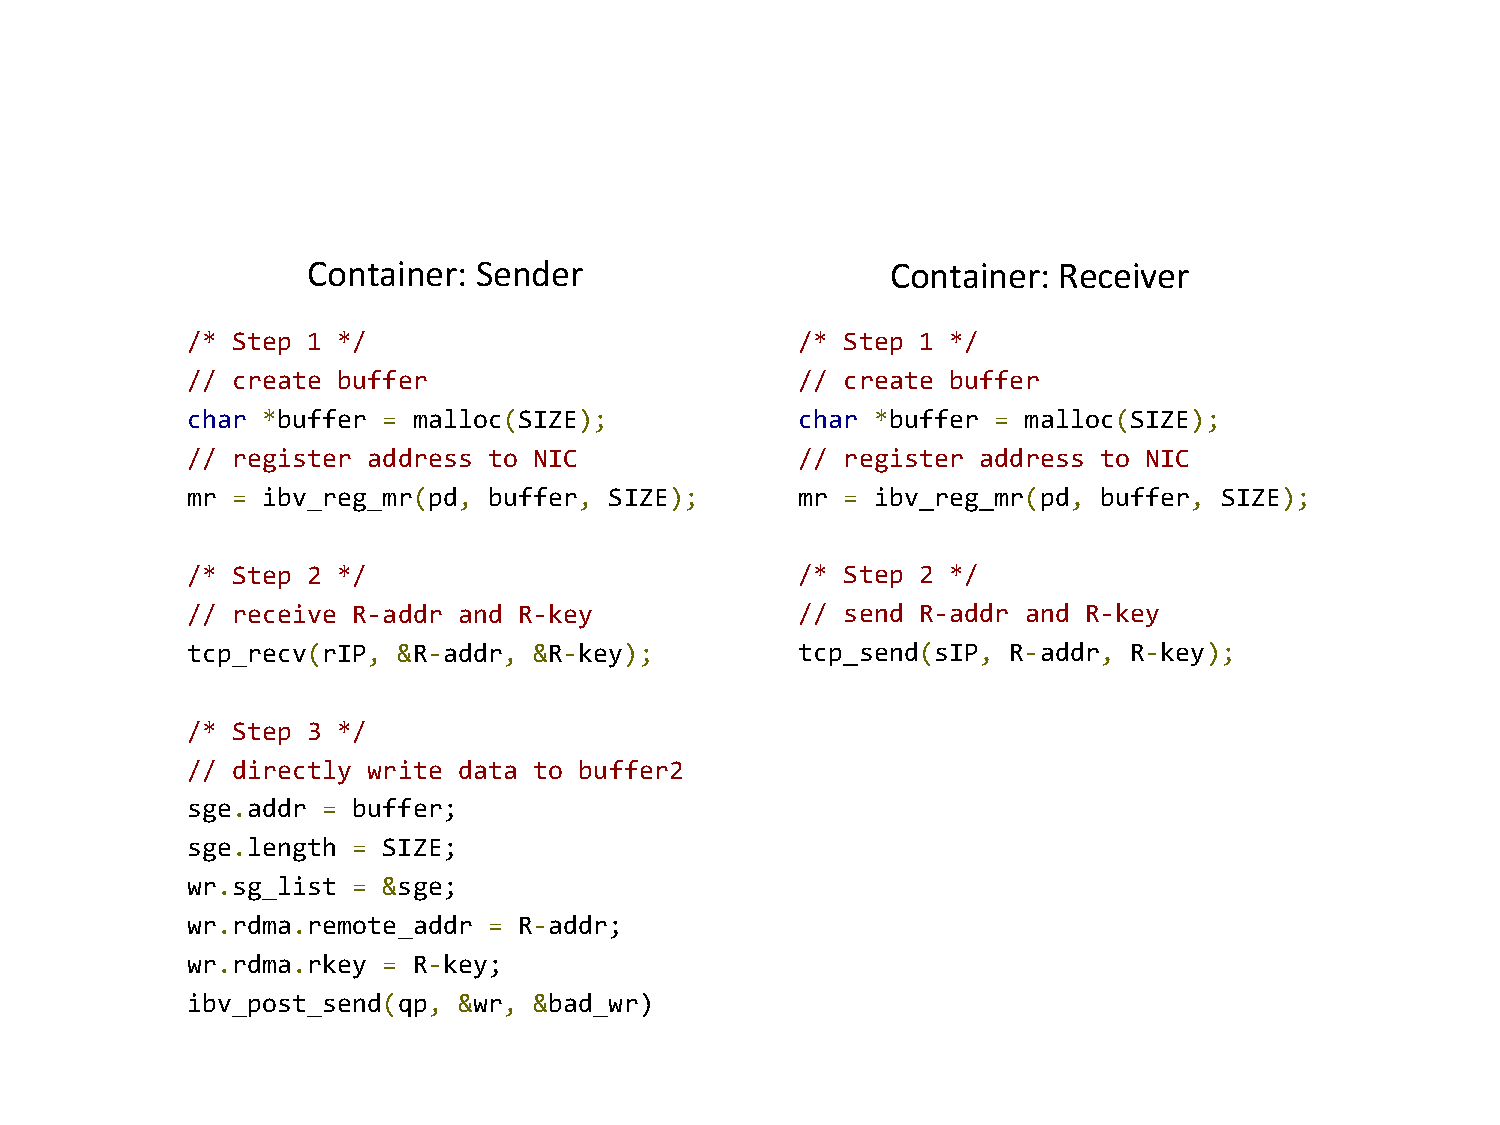
\includegraphics[width=0.45\textwidth]{figures/system/sys_rdma_code.pdf}      
     \label{fig:sys_rdma_code}
     \caption{The psudo code of an application execute RDMA write.} 
     \end{figure}

Figure XXX (a) shows the working flow of a standard RDMA write from containers'
points of view when they use Verbs API. There are generally three steps in a 
Write operation. 
Step 1: the sender first creates a memory block, puts data in it and passes 
the pointer of this memory block to its NIC;
Step 2: the sender notify its NIC to write the memory block to the receiver's IP.
Step 3: the receiver's NIC will get data from the sender's NIC and copy the 
data into a memory block and pass the pointer of the memory block to the 
receiver.

     \begin{figure}[ht]
     \centering 
     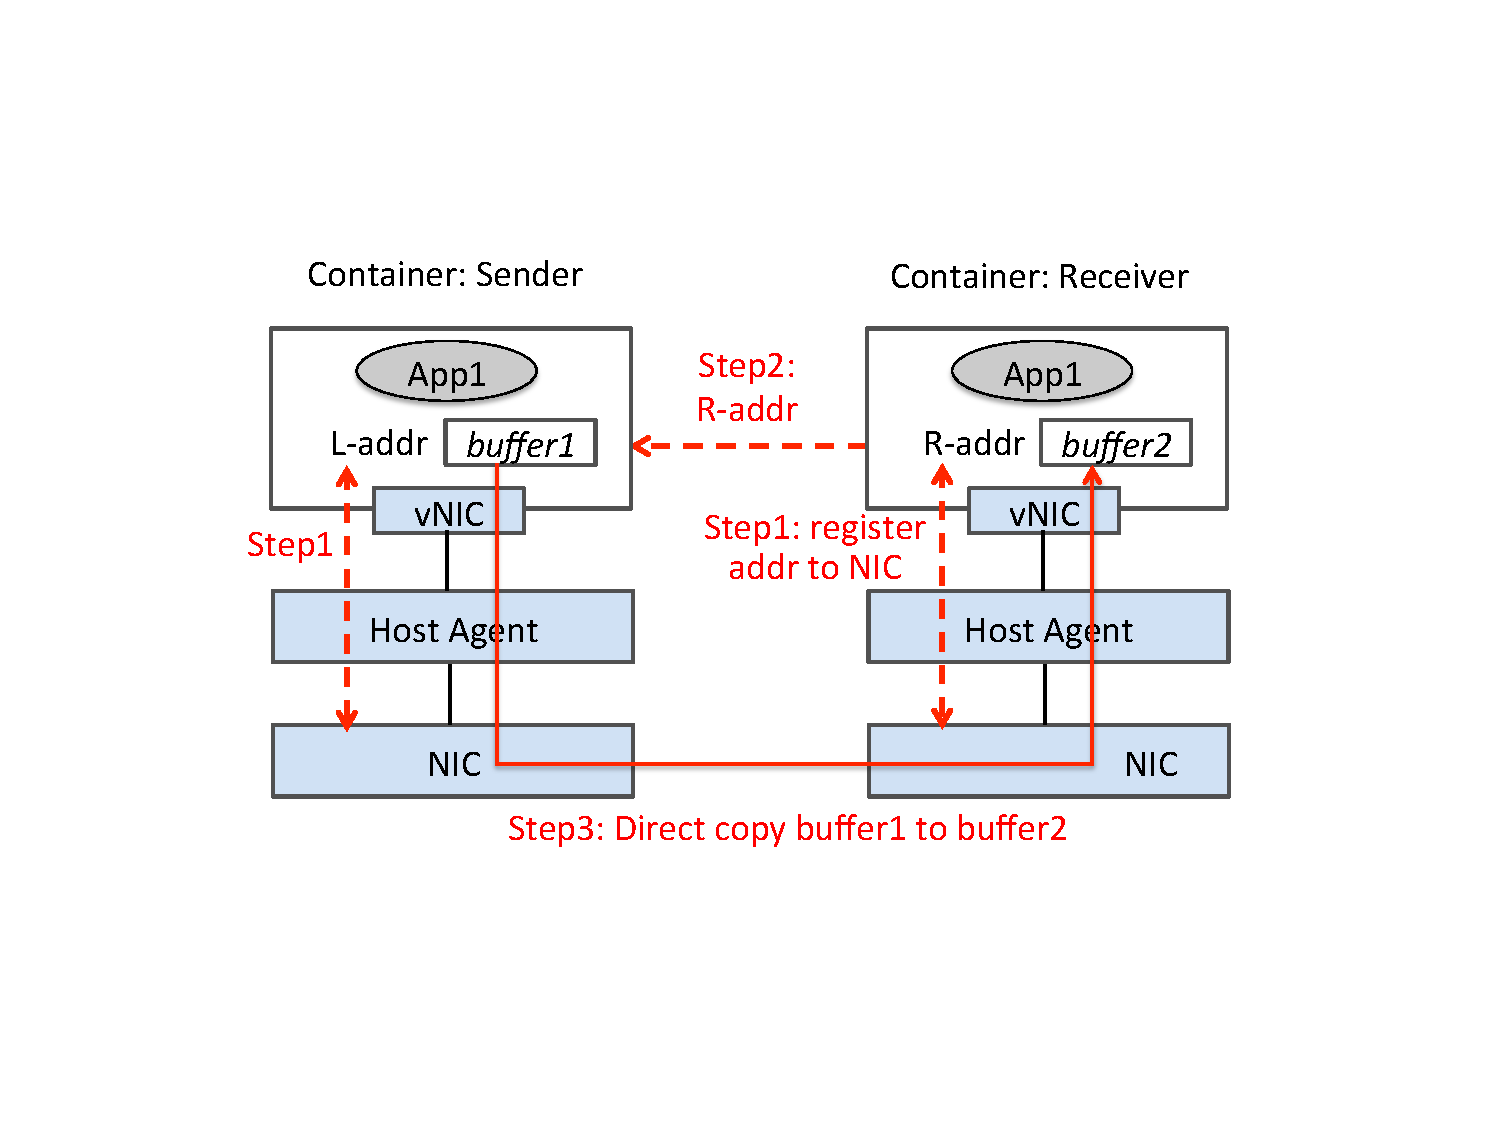
\includegraphics[width=0.45\textwidth]{figures/system/sys_rdma_rdma.pdf}      
     \label{fig:sys_rdma_rdma}
     \caption{How \sysname implemented RDMA write in inter-host setting.} 
     \end{figure}

In \sysname, both the sender and receiver containers have a virtual RDMA NIC.
In Step 1, the sender creates a shared-memory block and write data, and then 
the local network agent will get the pointer of this shared-memory block after the sender passes it to its virtual NIC; In Step 2, after receiving the IP of 
the receiver, the local network agent will check whether the receiver is on
the same host of the sender. If the answer is "Yes", the local network agent will
directly leverage the receiver's virtual NIC to notify it that a memory block 
from RDMA is ready to read with the pointer of the shared-memory block. 
Otherwise, the sender's local network agent will perform an actual RDMA write
with the receiver's local network agent, and the latter will put the received data into a shared-memory and pass it to the receiver container via its virtual NIC.
     
     \begin{figure}[ht]
     \centering 
     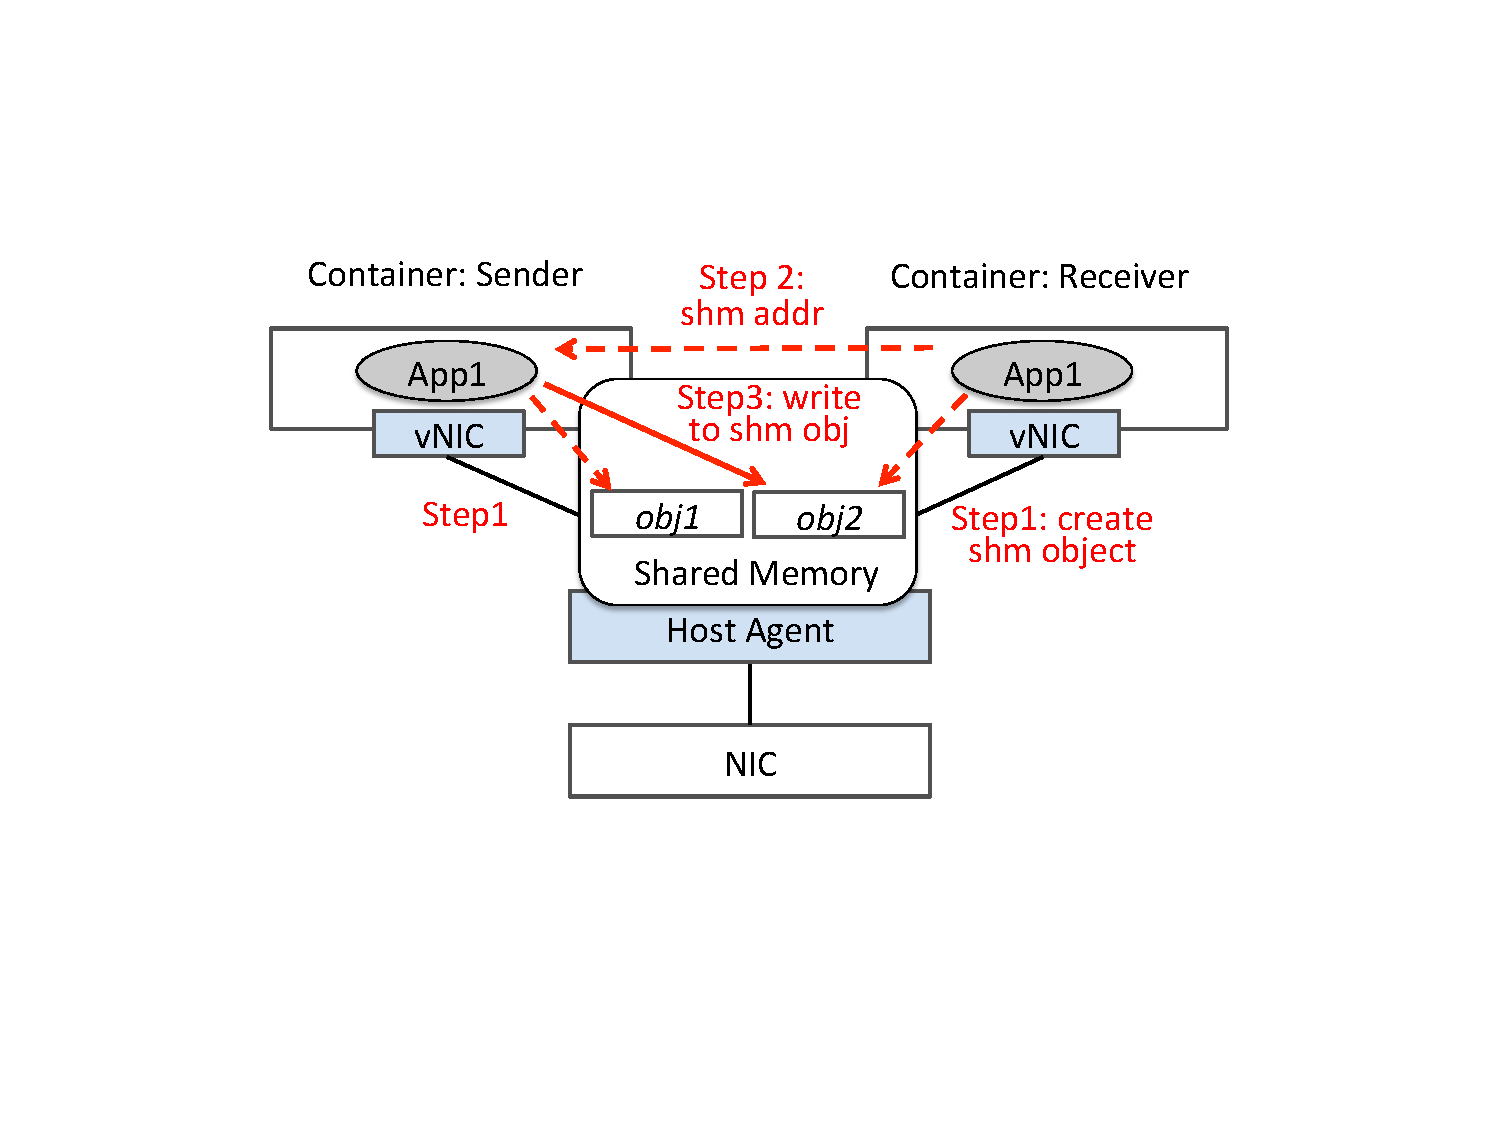
\includegraphics[width=0.45\textwidth]{figures/system/sys_rdma_shm.pdf}      
     \label{fig:sys_rdma_shm}
     \caption{How \sysname implemented RDMA write with shared memory in intra-host setting.} 
     \end{figure}
     


\iffalse

     \begin{figure}[ht]
     \centering 
     \begin{subfigure}
     \centering 
     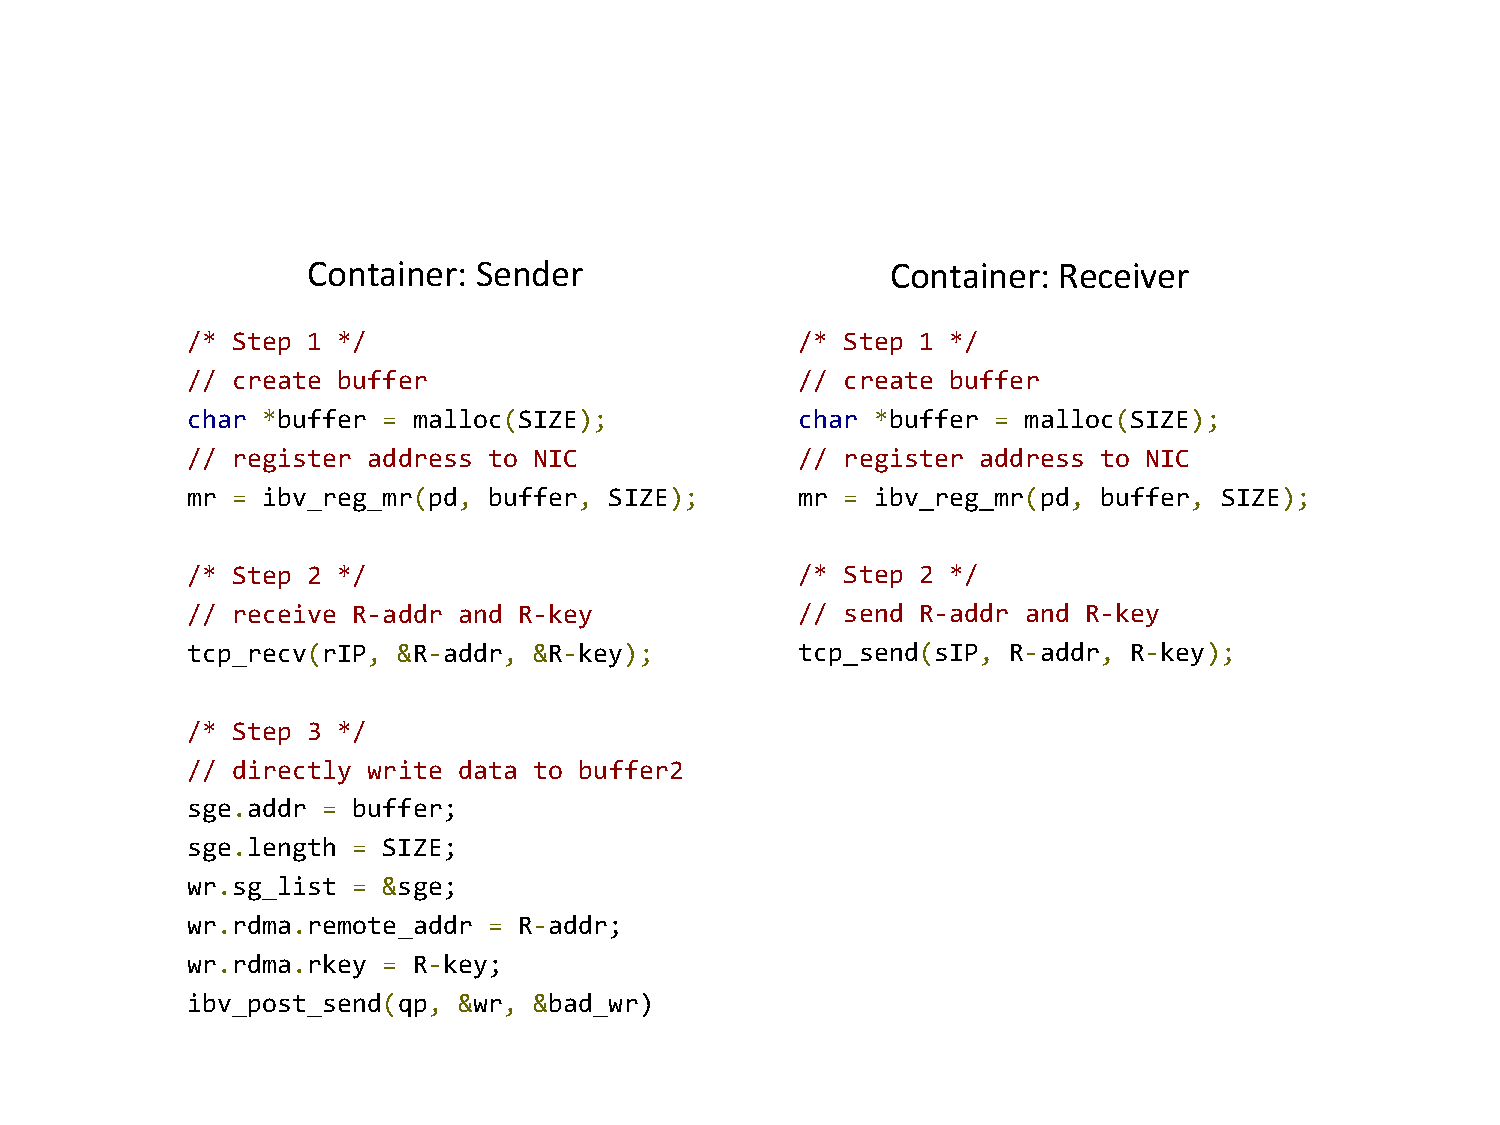
\includegraphics[width=0.45\textwidth]{figures/system/sys_rdma_code.pdf}
     %\caption{} 
     \end{subfigure}
           
     \begin{subfigure}
     \centering 
     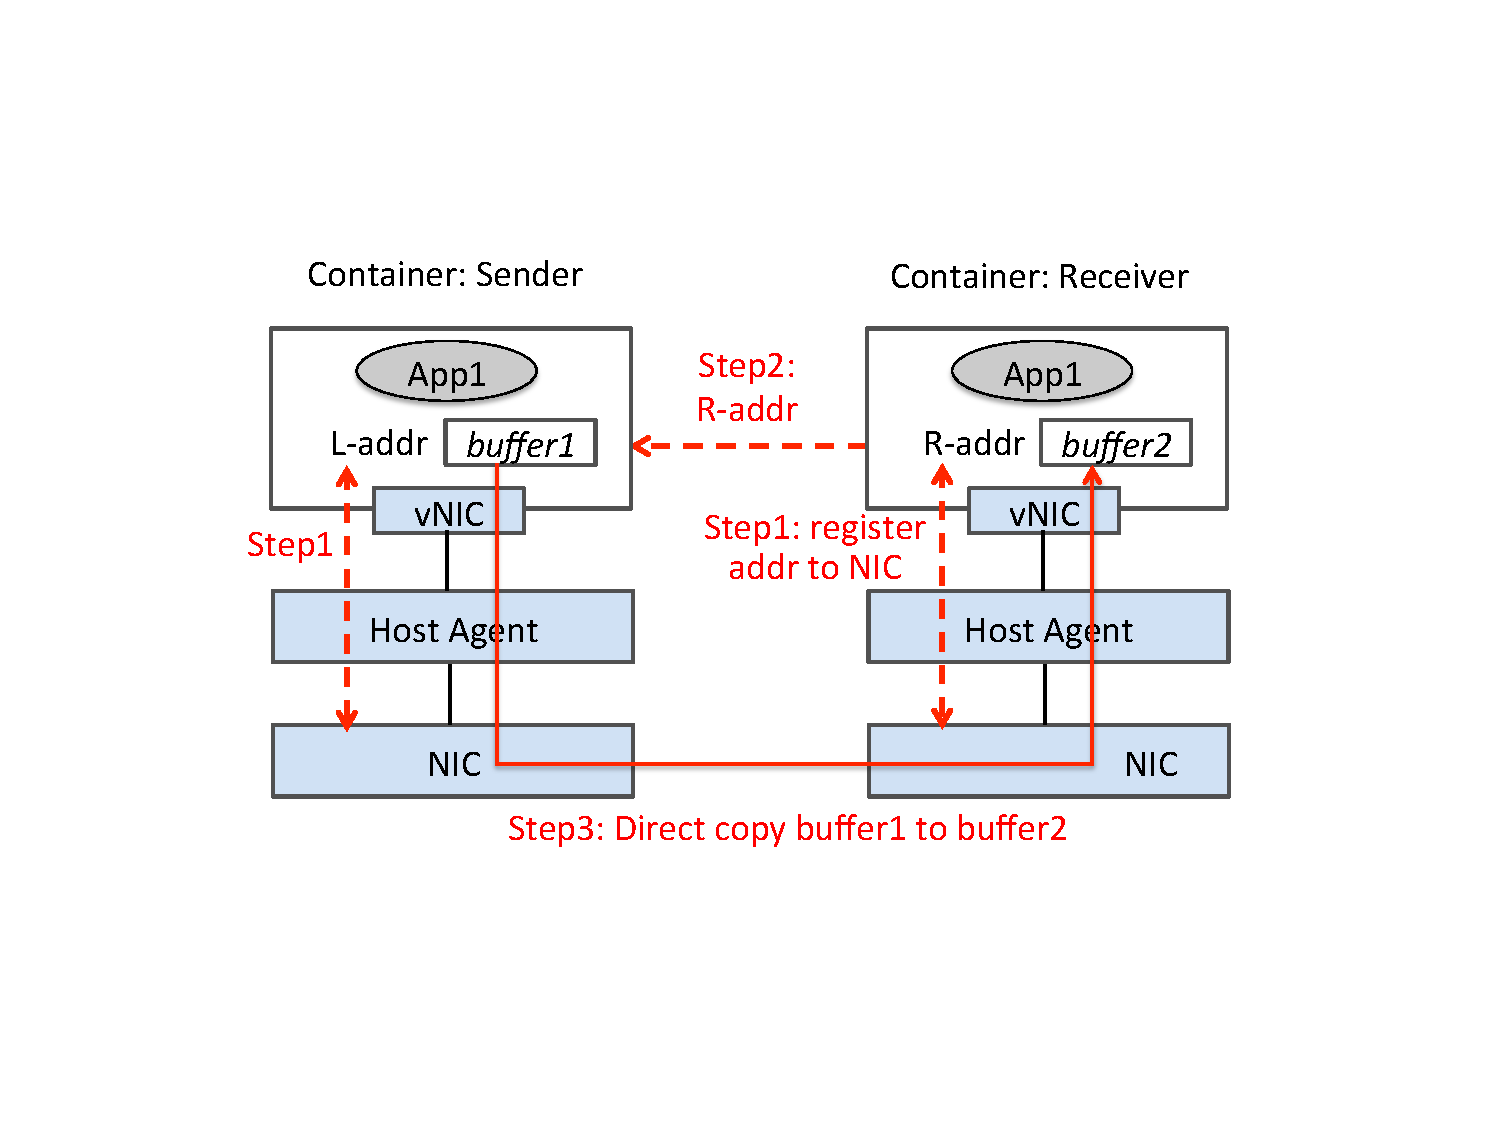
\includegraphics[width=0.45\textwidth]{figures/system/sys_rdma_rdma.pdf}      
     %\caption{} 
     \end{subfigure}
     
     \begin{subfigure}
     \centering
     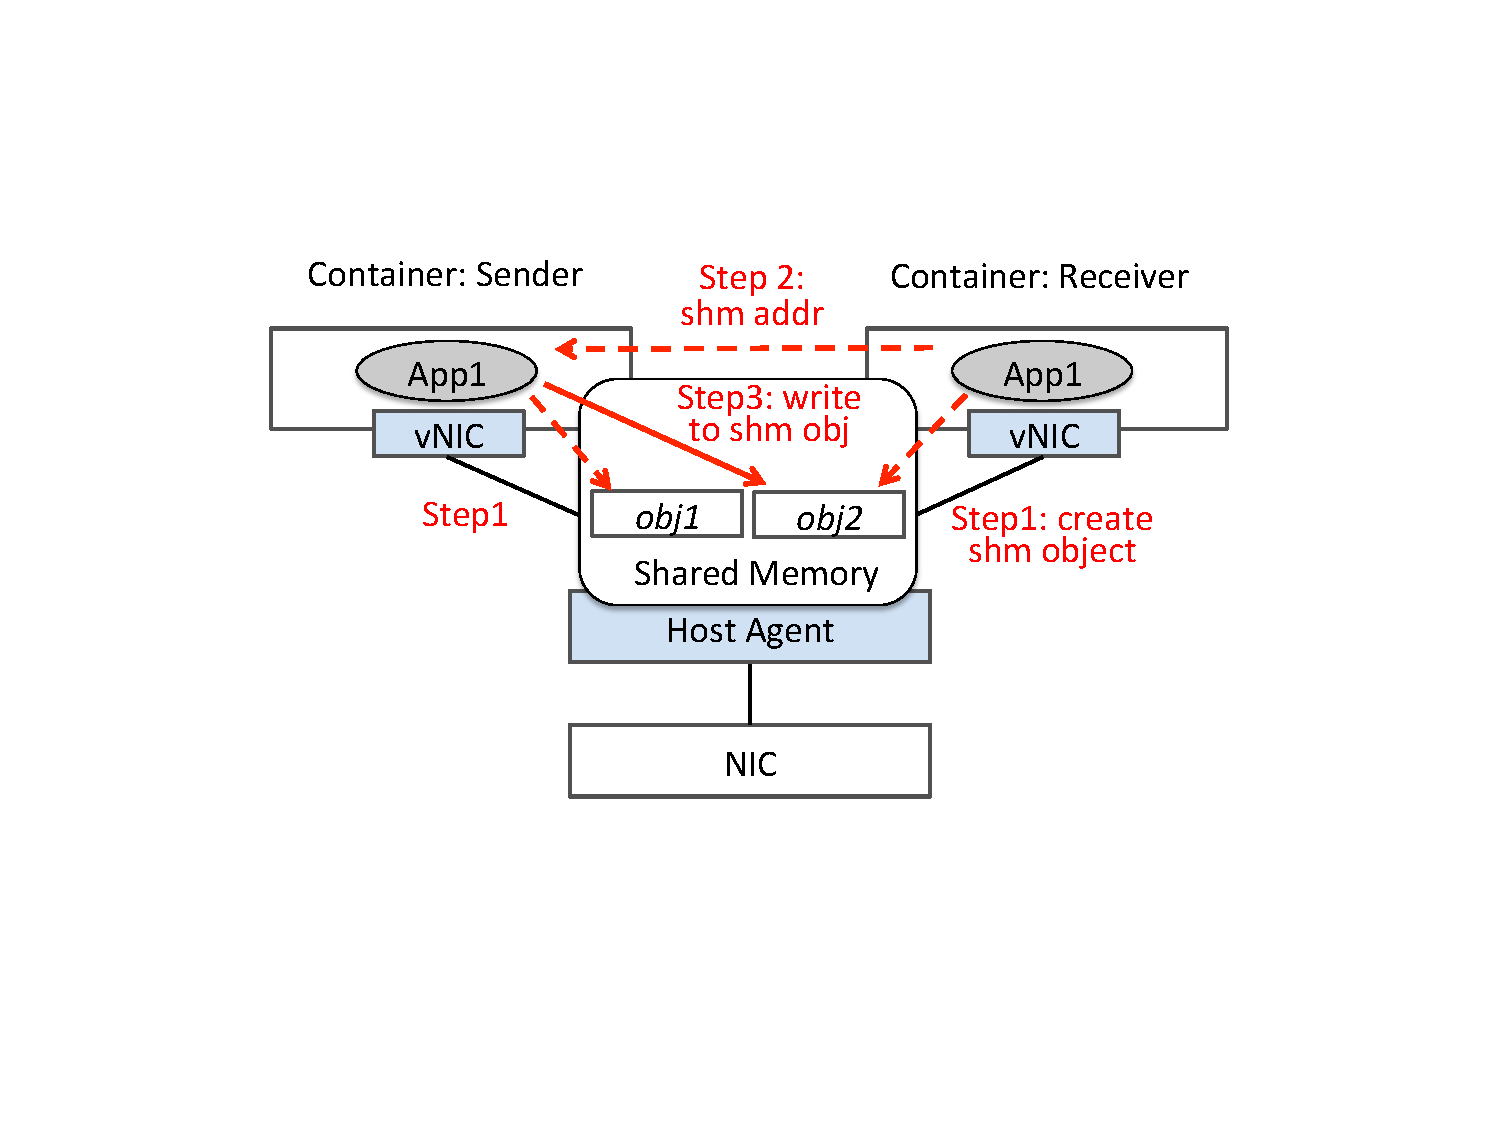
\includegraphics[width=0.45\textwidth]{figures/system/sys_rdma_shm.pdf}      
     %\caption{} 
     \end{subfigure}
     \label{fig:system_modules}
     \caption{The modules of \sysname.} 
     \end{figure}

%P1 introduce the two components we want to build
\sysname's main components includes a Orchestrator and a virtualized NIC.
The Orchestrator can figure out the most efficient way for two containers to talk with each other (e.g. 
via shared memory, rdma or dpdk) based on the location of the container or the resource
utilization of the host.
And the virtualized NIC emulates the necessary underlying resource structures 
(e.g., send queue or receive queue for RDMA). In this way, the application can
gain the desired \emph{portability}, since the application can now use the standardized  
APIs without being aware of the various underlying communication
mechanisms in different environments. 
Both of the components are shown in Figure~\ref{fig:system_modules}.

     \begin{figure}[ht]
     \centering 
     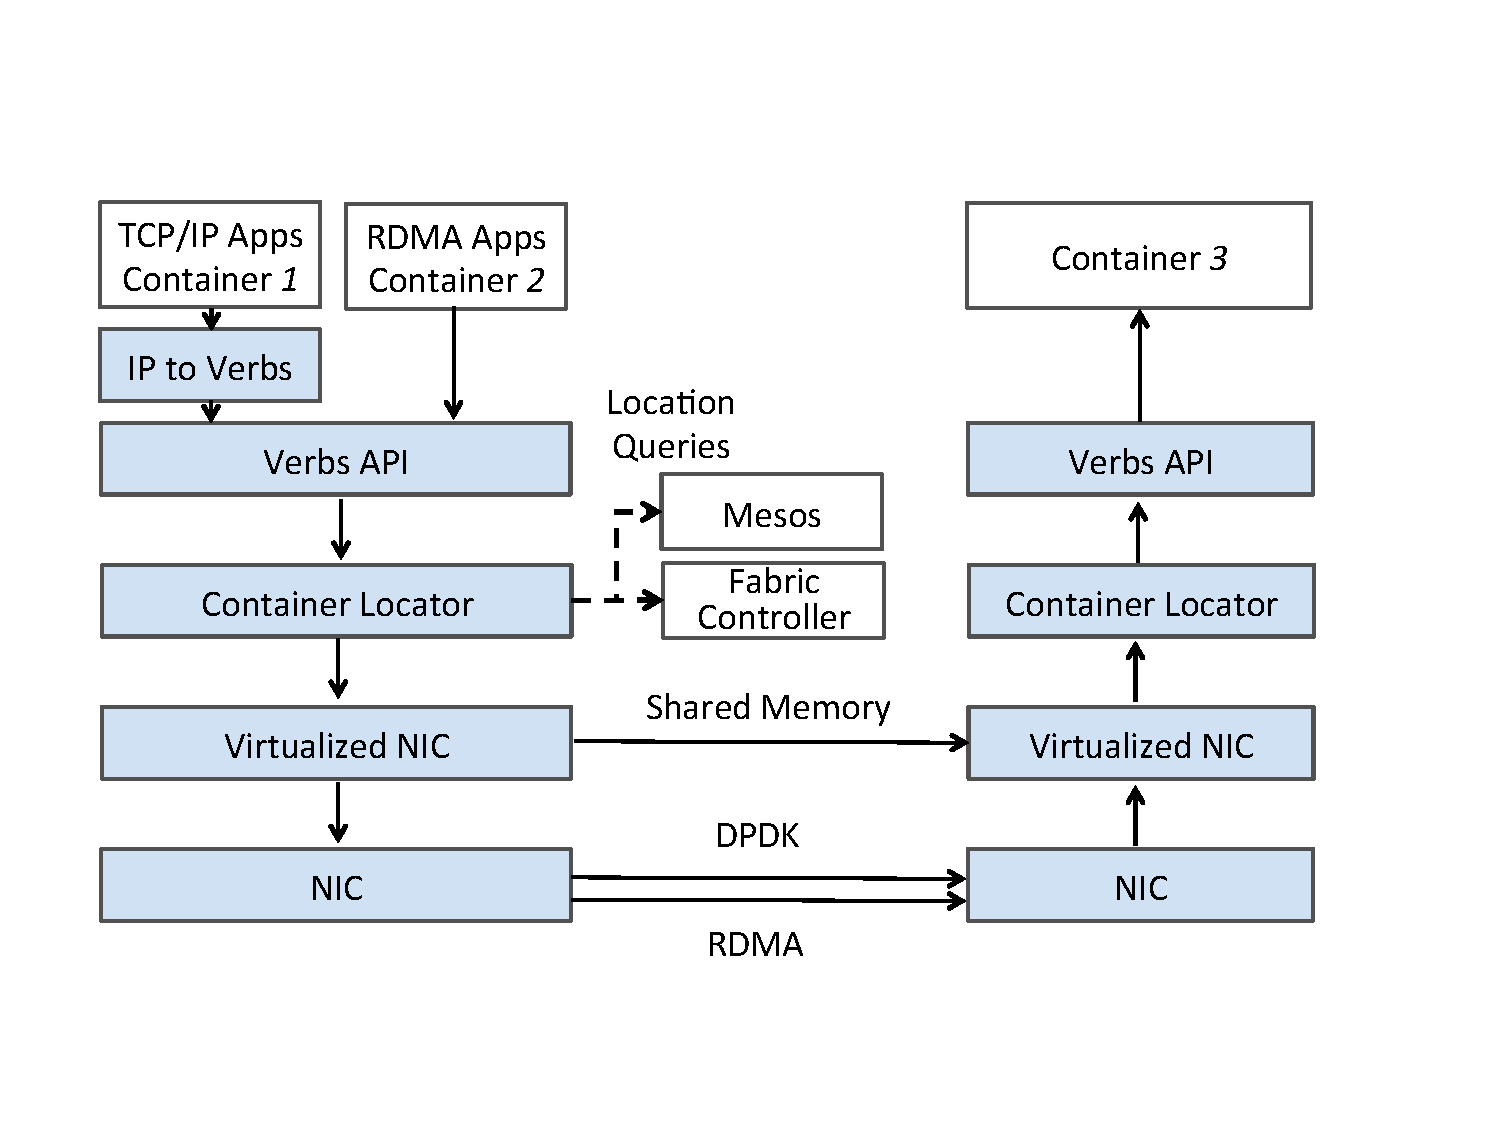
\includegraphics[width=0.45\textwidth]{figures/system/system_modules.pdf}      
     \label{fig:system_modules}
     \caption{The modules of \sysname.} 
     \end{figure}
     
      \begin{figure}[ht]
         \centering 
         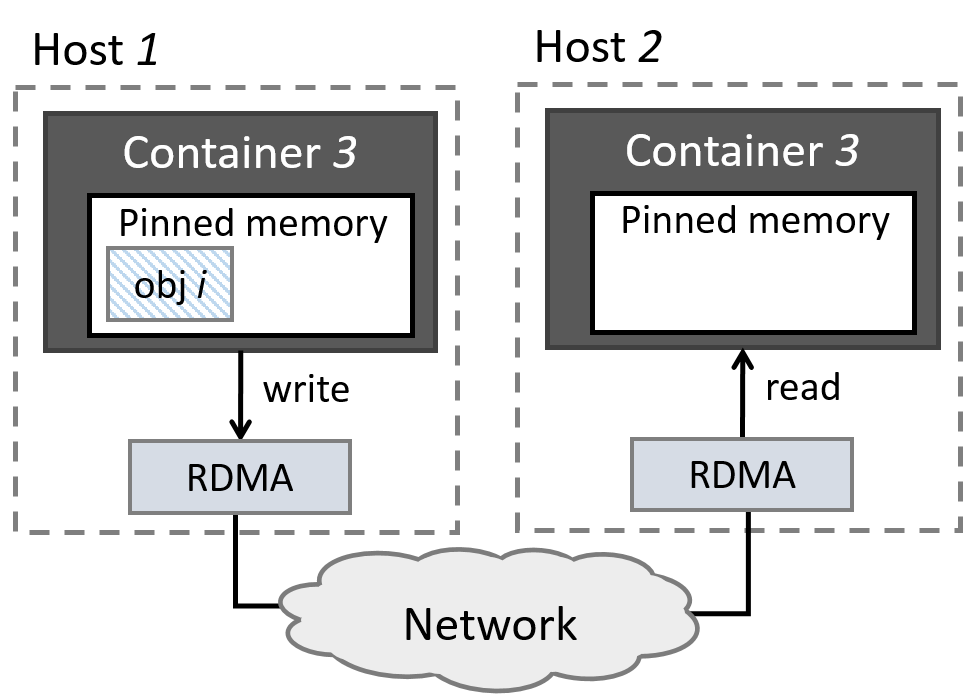
\includegraphics[width=0.2\textwidth]{figures/rdma-container.png}   
         \caption{??}   
      \end{figure}
      
      \begin{figure}[ht]
      	\centering 
      	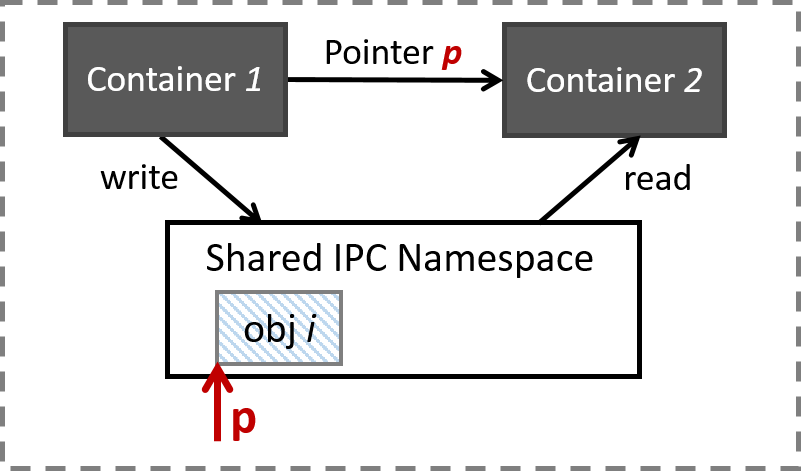
\includegraphics[width=0.2\textwidth]{figures/shared-mem-container.png}   
      	\caption{??}   
      \end{figure}

\subsection{Virtualized NIC}
The virtualized NIC (vNIC) a transparent layer between the application and the underlying network structure.
We modify the communication libraries of a container so the vNIC can intercept on the communication requests
from the applications (e.g. send request). For example, if the application is a RDMA application, we
will modify the library \texttt{libibverbs} to pass verbs calls to the vNIC.

The virtualized NIC has two roles. First, it queries the Orchestrator for the best mechanism to implement the 
communication requests, as illustrated in Figure~\ref{fig:system_modules}.
For example, if the two containers are intra-VM, it will create a shared namespace and memory objects 
for the two containers, and write the sender's data into the shared memory objects and pass the pointers of the
memory objects to the receiver container to transfer the data.

Second, the virtualized NIC (vNIC) emulates underlying network structure. 
For example, for RDMA, the vNIC will emulate the data structures including the Send Queue, 
Receive Queue, Completion Queue and Queue Pairs.
In this way, the vNIC not only maintains compatibility with currently written applications, but also
gain the desired \emph{portability}. Because the containers applications no longer need to bind to
the underlying network structure (bind to the vNIC instead), and the vNIC can be ported along with
the applications.

% as a emulation  underlying network structure
%a transparent layer between the application and the underlying network structure, dynamically choosing the best communication mechanism, while maintaining compatibility with currently written applications.

%The decision of which mechanism to chose is based on the hardware capabilities of the hosts and the physical placement of the containers, while aiming for minimal CPU overhead and high throughput. This decision and switching between communication mechanism is done completely transparent from application.

%For intra-host communication, virtualized NIC will use shared memory communication inducing minimal pressure on the CPU while reaching high throughput (~ memory bandwidth). For inter-host communication, the virtualized NIC will prioritize RDMA communication when supported by the underlying hardware. Otherwise, it will use TCP/IP communication. 


\subsection{Orchestrator}
The Orchestrator is a logic module to intelligently decide the most
efficient way to implement the communication request based on the locations
of the containers or the resources utilization of the host.

     \begin{figure}[ht]
     \centering 
     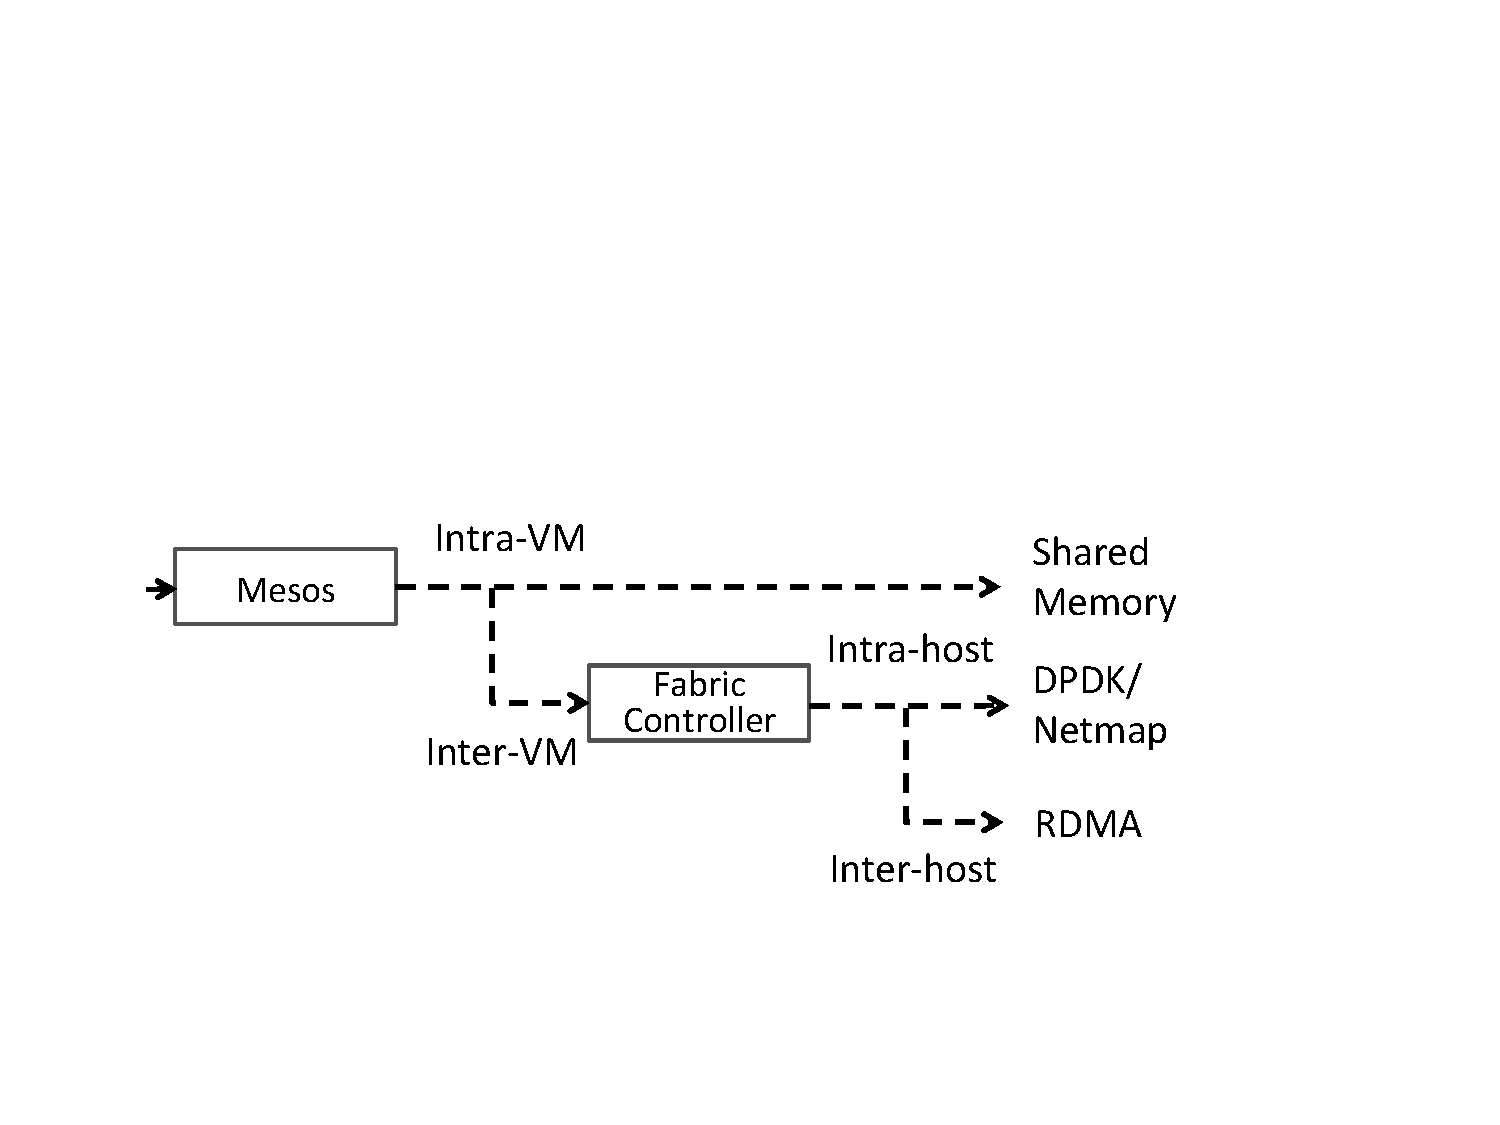
\includegraphics[width=0.45\textwidth]{figures/system/system_locator.pdf}      
     \label{fig:system_locator}
     \caption{The logic flow of Orchestrator.} 
     \end{figure}

Suppose the decision is only based on the location of the containers, the logic will be as follows.
The Orchestrator send queries to Mesos (resource manager) and the cloud's Fabric Controller to locate
the sender/receiver containers and decide the most efficient way they talk with each other.
The logic flow of this process is as shown in Figure~\ref{fig:system_locator}.
For example, given a send request, the Orchestrator will query Mesos to figure out if the 
sender/receiver containers are intra-VM or inter-VM. 
For intra-VM containers, the Orchestrator will raise a flag to notify the virtualized NIC to
send the data via shared memory.
For inter-VM containers, the Orchestrator will then quire if the two containers are intra-host
or inter-host.
If the containers are inter-VM but intra-host, Orchestrator will tell the virtualized NIC to send
the data via fast data pass across VMs in the same machine, such as NetVM\cite{} or netmaps\cite{}.
Or if the containers are inter-host, RDMA would be the most efficient way to perform the data transfer.

\tianlong{There should be some design decisions to support the above logic in design section.}

%We are going to add a logic module called Orchestrator inside the application's
%library for communication. For example, the  

\subsection{Put It Together}
Now let's put the components together and see the workflow of \sysname, as shown in Figure~\ref{fig:system_modules}.
Let's take two rdma applications (in container2 and container3) as an example.
Suppose application in container2 (app2 in short) issues a send data to container3 request via standardized Verbs API.
The vNIC will intercept the request and query the Orchestrator. 
Then the orchestrator will query Mesos or Fabric Controller to obtain the locations of 
container2 and container3. Then Orchestrator will send a decision of the best mechanism to the vNIC.
The request will call to the emulated data structures in the vNIC (e.g. QP, SQ, RQ, CQ). And the vNIC will choose the
best mechanism (e.g. RDMA, shared memory, dpdk/netmap) to implement the request. For example, if the containers
are inter-host, RDMA will be selected. If the best mechanism is not available (e.g. NIC lack of RDMA support), it will
fall back to the sub-optimal mechanism (e.g., TCP/IP).

\fi